\documentclass[a4paper]{article}

%% Language and font encodings
\usepackage[english]{babel}
\usepackage[utf8x]{inputenc}
\usepackage[T1]{fontenc}

\usepackage{tikz}
\usetikzlibrary{matrix}
\usepackage{algpseudocode} 

%% Sets page size and margins
\usepackage[a4paper,top=3cm,bottom=2cm,left=3cm,right=3cm,marginparwidth=1.75cm]{geometry}
\usepackage{amsmath}
\usepackage{amsthm}
\usepackage{amssymb}

\newtheorem{theorem}{Theorem}
\newtheorem{lemma}[theorem]{Lemma}

\begin{document}
\section*{Randomized min-cut algorithm}
Consider the randomized min-cut algorithm discussed in class.
We have seen that its probability of success is at least $1 / \binom{n}{2}$, where $n$ is the number of its vertices.
\begin{itemize}
\item Describe how to implement the algorithm when the graph is represented by adjacency lists, and analyze its running time.
In particular, a contraction step can be done in $O(n)$ time.
\item A weighted graph has a weight $w(e)$ on each edge $e$, which  is  a  positive  real number.
The  min-cut  in  this  case  is  meant  to  be  min-weighted  cut,  where  the sum  of  the  weights  in  the  cut  edges  is  minimum.
Describe  how  to  extend  the algorithm  to  weighted  graphs,  and  show  that  the  probability  of  success  is  still $\geq 1/\binom{n}{2}$. [hint: define the weighted degree of a node]
\item Show that running the algorithm multiple times independently at random, and taking the minimum among the min-cuts thus produced, the probability of success can be made at least $1 - 1/n^c$ or a constant $c > 0$ (hence, with high probability).
\end{itemize}
\
\\
\\
\textbf{SOLUTION}
\\
\\

\noindent
\textbf{First Point}
\\
In order to solve this point, we use two data structure, pre-processed, to have linear access on the data. The graph is saved as a sorted adjacency list but, instead saving in a list one entry for each edge, we will save a cell that contains the edge ID and its multiplicity. 

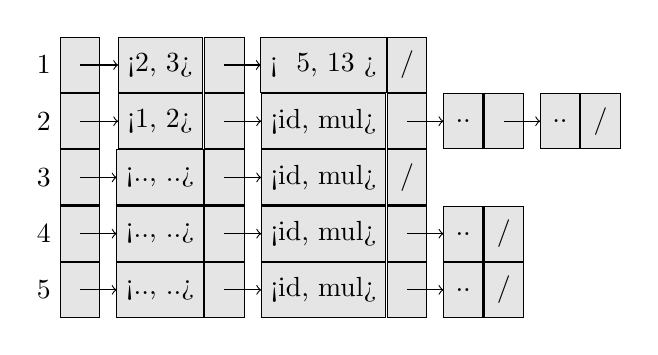
\begin{tikzpicture}
\matrix (M) [matrix of nodes,
column sep=0pt,
row sep=0pt,
nodes={draw,fill=gray!20,minimum width=.5cm,outer sep=0pt,minimum
height=.7cm,anchor=center},
column 1/.style={minimum height=.8cm}]{
 \mbox{} &[2mm] <2, 3> & \mbox{} &[2mm] < \ 5, 13   > & $/$  &[2mm]   &   &[2mm]   & \\
 \mbox{} & <1, 2> & \mbox{} & <id, mul> & \mbox{}  & .. &  \mbox{} & .. & $/$  \\
 \mbox{}  & <.., ..>  & \mbox{} & <id, mul> & $/$  &   &   &   & \\
 \mbox{} & <.., ..> & \mbox{} & <id, mul> & \mbox{}  & .. & $/$  &   & \\
 \mbox{} & <.., ..> & \mbox{} & <id, mul> & \mbox{}  & .. & $/$  &   & \\
};
\foreach \i in {1,2,3,4,5}{
\path (M-\i-1) [late options={label=left:\i}];
\draw[->] (M-\i-1.center)--(M-\i-2.west);
\draw[->] (M-\i-3.center)--(M-\i-4.west);
}
\draw[->] (M-2-5.center)--(M-2-6.west);
\draw[->] (M-4-5.center)--(M-4-6.west);
\draw[->] (M-5-5.center)--(M-5-6.west);
\draw[->] (M-2-7.center)--(M-2-8.west);
\end{tikzpicture}

Another data structure that we will use is a \textit{Virtual Table} $V_T$. $V_T$ is an array of size $n$ initialized so that 
$$ \forall i \in [n].\ V_t[i]=i$$
Suppose we decide to contract the edge $(i,j)$: in line of principle, this would replace nodes $i$ and $j$ with a new node $n_{ij}$; however, we will will rather collapse node $j$ \emph{into} $i$ ($n_{ij} = i$) by setting $V_T[j] := i$ (and properly updating the adjacency list for $i$).

Throughout the algorithm, $V_T$ will thus accumulate a number of node redirections (aliases).
\\

\noindent
\textit{Random choice of edge}\\
Let $N$ be the initial number of nodes, $n$ be the number of remaining unique nodes.

Let $M$ be the initial number of edges, $m$ be the number of remaining edges.

Let $\Delta$ be an array of $N$ elements, each containing $\delta(i)$, the degree of node $i$ (NB: contracted nodes will have degree 0). Then:\\


\begin{algorithmic}
\Function{ChooseEdge}{}
\State $r \gets rand(0, 2m-1)$ \Comment{note $\sum_{i=1}^{n}\delta(i) = 2m$}
\State $i = 0$ \
\While {$\Delta[i] < r$}
	\State $r \gets r - \Delta[i]$
	\State $i \gets i + 1$
\EndWhile
\State $j = 0$
\While {$nodes[i].adj[j].mult < r$}
	\State $r \gets r - nodes[i].adj[j].mult$
	\State $j \gets j + 1$
\EndWhile
\State \Return $(i,\ V_T[j])$
\State
\EndFunction
\end{algorithmic}

You can think of what we're doing as having concatenated the adjacency lists and then crawled through them to edge $r$. This would require $O(n^2)$ steps done naively, but saving the degree of the node (the length of the adjacency list) allows us to skip to the next done in one step (a sort of skip-pointer).
\\

This procedures results in a random uniform choice of the edge. In fact, the chance that a specific (directed!) edge $(i, j)_k$ is chosen ends up being:
$$P_r[(i,j_k)] = \frac{\delta(i)}{2 \times m} \times \frac{mult(i,j)}{\delta(i)} \times \frac{1}{mult(i,j)} = \frac{1}{2 \times m}$$
where
$$\frac{\delta(i)}{2 \times m} = P_r[node\ i\ is\ chosen]$$
$$\frac{mult(i,j)}{\delta(i)} = P_r[\{(i,j)_k\}|\ node\ i]$$
$$\frac{1}{mult(i,j)} = P_r[(i,j)_k|\ \{(i,j)_k\}]$$
$$\{(i,j)_k\}\ \text{is the set of all edges going from i to j}$$
$$mult(i,j) = |\{(i,j)_k\}|\ \text{is the multiplicity of edge (i,j)}$$
\\

Thus, the probability that an (undirected!) edge $(i,j)_k$ is chosen results
$$\frac{1}{2m} + \frac{1}{2m} = \frac{1}{m}$$
\\
\noindent
\textit{Contraction}\\
To merge two nodes $i$ and $j$ we need to scroll the lists of the merging nodes and, assuming the ordered data, we can merge into one list in $O(2n) = O(n)$ (whenever $i$ and $j$ both point to a third node $k$, i.e. there are edges $(i,k),\ (j,k)$, the multiplicity of the new edges $(n_{ij},k)$ and $(k, n_{ij}$) will be the sum of the multiplicities of $(i,k)$ and $(j,k)$).

It is also necessary to appropriately update $V_T$ and $\Delta$.
\\
\\

\noindent
\textbf{Second Point}
\\

In the algorithm we change the way we choose an edge to contract: edges with high weight will have a greater probability to be chosen with respect to others with lower weight.
We define $weight: E \longrightarrow \mathbb{R}$ as the function that associate the weight to a given edge.
We will use the $weight$ function also on subsets of $E$, intending for $weight(X)$ with $X \subseteq E$ the sum of the weight of all the edges in $X$.
\begin{align*}
&weight(X) = \sum_{e \in X} weight(e) &where\ X \subseteq E
\end{align*}
As seen in class, the \textit{min cut} is not unique, nevertheless the sum of weights in all \textit{min\_cuts} is the same, than with a notation abuse we will call it $weight(min\_cut)$.
For each edge $x \in E$ the probability to be choose for a contraction is given by its weights normalized with the total sum of the weights of all the edges of the graph.
\begin{align*}
Pr[extract\ x] = \frac{weight(x)}{weight(E)}\\
\end{align*}
Now the probability of making an error, when extracting an edge at random, is the probability of extracting one of the ``bad'' edges, i.e. edges such that their contraction cause a variation in $weight(min\_cut)$.
We name $BAD$ the set of ``bad'' edges.
\begin{align*}
&Pr[error] = \sum_{e \in BAD} Pr[extract\ e] = \sum_{e \in BAD} \frac{weight(e)}{weight(E)} = \frac{weight(BAD)}{weight(E)} \tag{1}
\end{align*}
As usual bad edges are those belonging to every \textit{min cut}, so the total weight of bad edges is less or equal to the weight of \textit{min cut}.
\begin{align*}
&weight(BAD) \leq {weight(min\_cut)} \tag{2}
\end{align*}
Given a node $v$, we define $star(v)$ as the set of all the edges touching $v$.
For the same reasons explained in class, for each node $v$ the weight of \textit{min cut} must be less or equal to the sum of the weights of the edges touching $v$.
This is because otherwise we would have a cut, $star(n)$, with weight less than \textit{min cut}, which is absurd.
\begin{align*}
&\forall\ v \in V\ .\ weight(min\_cut) \leq weight(star(v)) \tag{3}
\end{align*}
We can reformulate the \textit{handshaking lemma} for weighted graph in the following way, in which $weight(star(v))$ is something like the ``weighted degree'' of the node $v$.
\begin{align*}
weight(E) = \frac{\sum_{v \in V} weight(star(v))}{2} \tag{4}
\end{align*}
Now we can derive:
\begin{align*}
weight(E) &= \frac{\sum_{v \in V} weight(star(v))}{2} \tag{from 4}\\
&\geq \frac{\vert V \vert weight(min\_cut)}{2} \tag{from 3}\\ \\
weight(min\_cut) &\leq \frac{2\ weight(E)}{\vert V \vert} \tag{5}
\end{align*}
Finally we have all the ingredients for the proof:
\begin{theorem}
Selecting the edges for the contraction according to the probability described, each time we choose an edge the probability of choosing a ``bad'' edge is less or equal than $2 / \vert V \vert$.
\begin{align*}
Pr[error] \leq \frac{2}{\vert V \vert}
\end{align*}
\end{theorem}
\begin{proof}
\begin{align*}
Pr[error] &= \frac{weight(BAD)}{weight(E)} \tag{from 1}\\
&\leq \frac{weight(min\_cut)}{weight(E)} \tag{from 2}\\
&\leq \frac{\frac{2\ weight(E)}{\vert V \vert}}{weight(E)} \tag{from 5}\\
&= \frac{2\ weight(E)}{\vert V \vert weight(E)} = \frac{2}{\vert V \vert}
\end{align*}
\end{proof}
The probability of making an error when selecting an edge is the same as for the case of a normal graph seen in class, so the probability of success for the algorithm (i.e. the probability of choosing well all the times) is still $\geq 1/ \binom{n}{2}$.
\\
\\
\noindent
\textbf{Third Point}
\\

We know that $P(n) \geq 1 / \binom{n}{2}$ is the probability of choose well for $N$ times.
We have seen also that the probability of error is $\leq (1 - 1/\binom{n}{2})$.
Then the probability of having an error each time in $N$ repetitions of the algorithm is 
\begin{align*}
leq (1 - \frac{1}{\binom{n}{2}})^N \approx e^{-\frac{2N}{n(n-1)}}
\end{align*}

Given a $c$ we want the probability of success to be $\geq 1 - 1/n^c$.
This is equivalent to ask that the probability of error is $\leq 1/n^c$.
Making some calculations:
\begin{align*}
\frac{1}{e^{\frac{2N}{n(n-1)}}} = e^{-\frac{2N}{n(n-1)}} &\leq \frac{1}{n^c}\\
n^c &\leq e^{\frac{2N}{n(n-1)}}\\
ln(n^c) &\leq ln(e^{\frac{2N}{n(n-1)}}) = \frac{2N}{n(n-1)}\\
N \geq \frac{n(n-1)ln(n^c)}{2}
\end{align*}
So, for each given $c$, to make the probability of success at least $1 - 1/n^c$ is sufficient to take $N$ grater or equal than $\frac{1}{2} n(n-1)ln(n^c)$.

\end{document}